%!TEX root = ../template.tex
%%%%%%%%%%%%%%%%%%%%%%%%%%%%%%%%%%%%%%%%%%%%%%%%%%%%%%%%%%%%%%%%%%%
%% chapter1.tex
%% NOVA thesis document file
%%
%% Chapter with introduction
%%%%%%%%%%%%%%%%%%%%%%%%%%%%%%%%%%%%%%%%%%%%%%%%%%%%%%%%%%%%%%%%%%%

\typeout{NT FILE chapter1.tex}

\chapter{Introduction}
\label{cha:introduction}

\prependtographicspath{{Chapters/Figures/Covers/}}

% epigraph configuration
\epigraphfontsize{\small\itshape}
\setlength\epigraphwidth{12.5cm}
\setlength\epigraphrule{0pt}

\epigraph{
  This work is licensed under the \href{LaTeX project public license}{\LaTeX\ Project Public License v1.3c}.
  To view a copy of this license, visit \url{LaTeX project public license}.
}

This is the \novathesis\ \LaTeX\ template version v\novathesisversion\ from \novathesisdate.

\section{If You Use this Template…} 
\label{sub:if_you_use_this_template}

This Chapter presents an introduction to the template and how it is organized. In the next chapter you can find some specific instructions. Please read the next sections carefully.

Someone spent a few dozens of hours working on this template to make your life easier and to allow you to be more productive.  Those working hours were not paid and were “stolen” from family.
If you use this template, please go to the
\href{https://github.com/joaomlourenco/novathesis_word}{project web page in GitGub}
and:
\begin{enumerate}
  \item Cite it~\cite{novathesis-manual} in your thesis/disseration with “\verb!\cite{novathesis-manual}!”, any place you think it makes sense.  If you cite it this way, the correct entry will be added automatically to your bibliography (there no need to add it to your BibTeX file);
  \item Give the project a star (marked with a red ellipse at the top-right in Figure~\ref{fig:github}); and
  \item Make a small donation (marked with a red ellipse at the bottom-left in Figure~\ref{fig:github}).
\end{enumerate}

\begin{figure}[htbp]
  \centering
    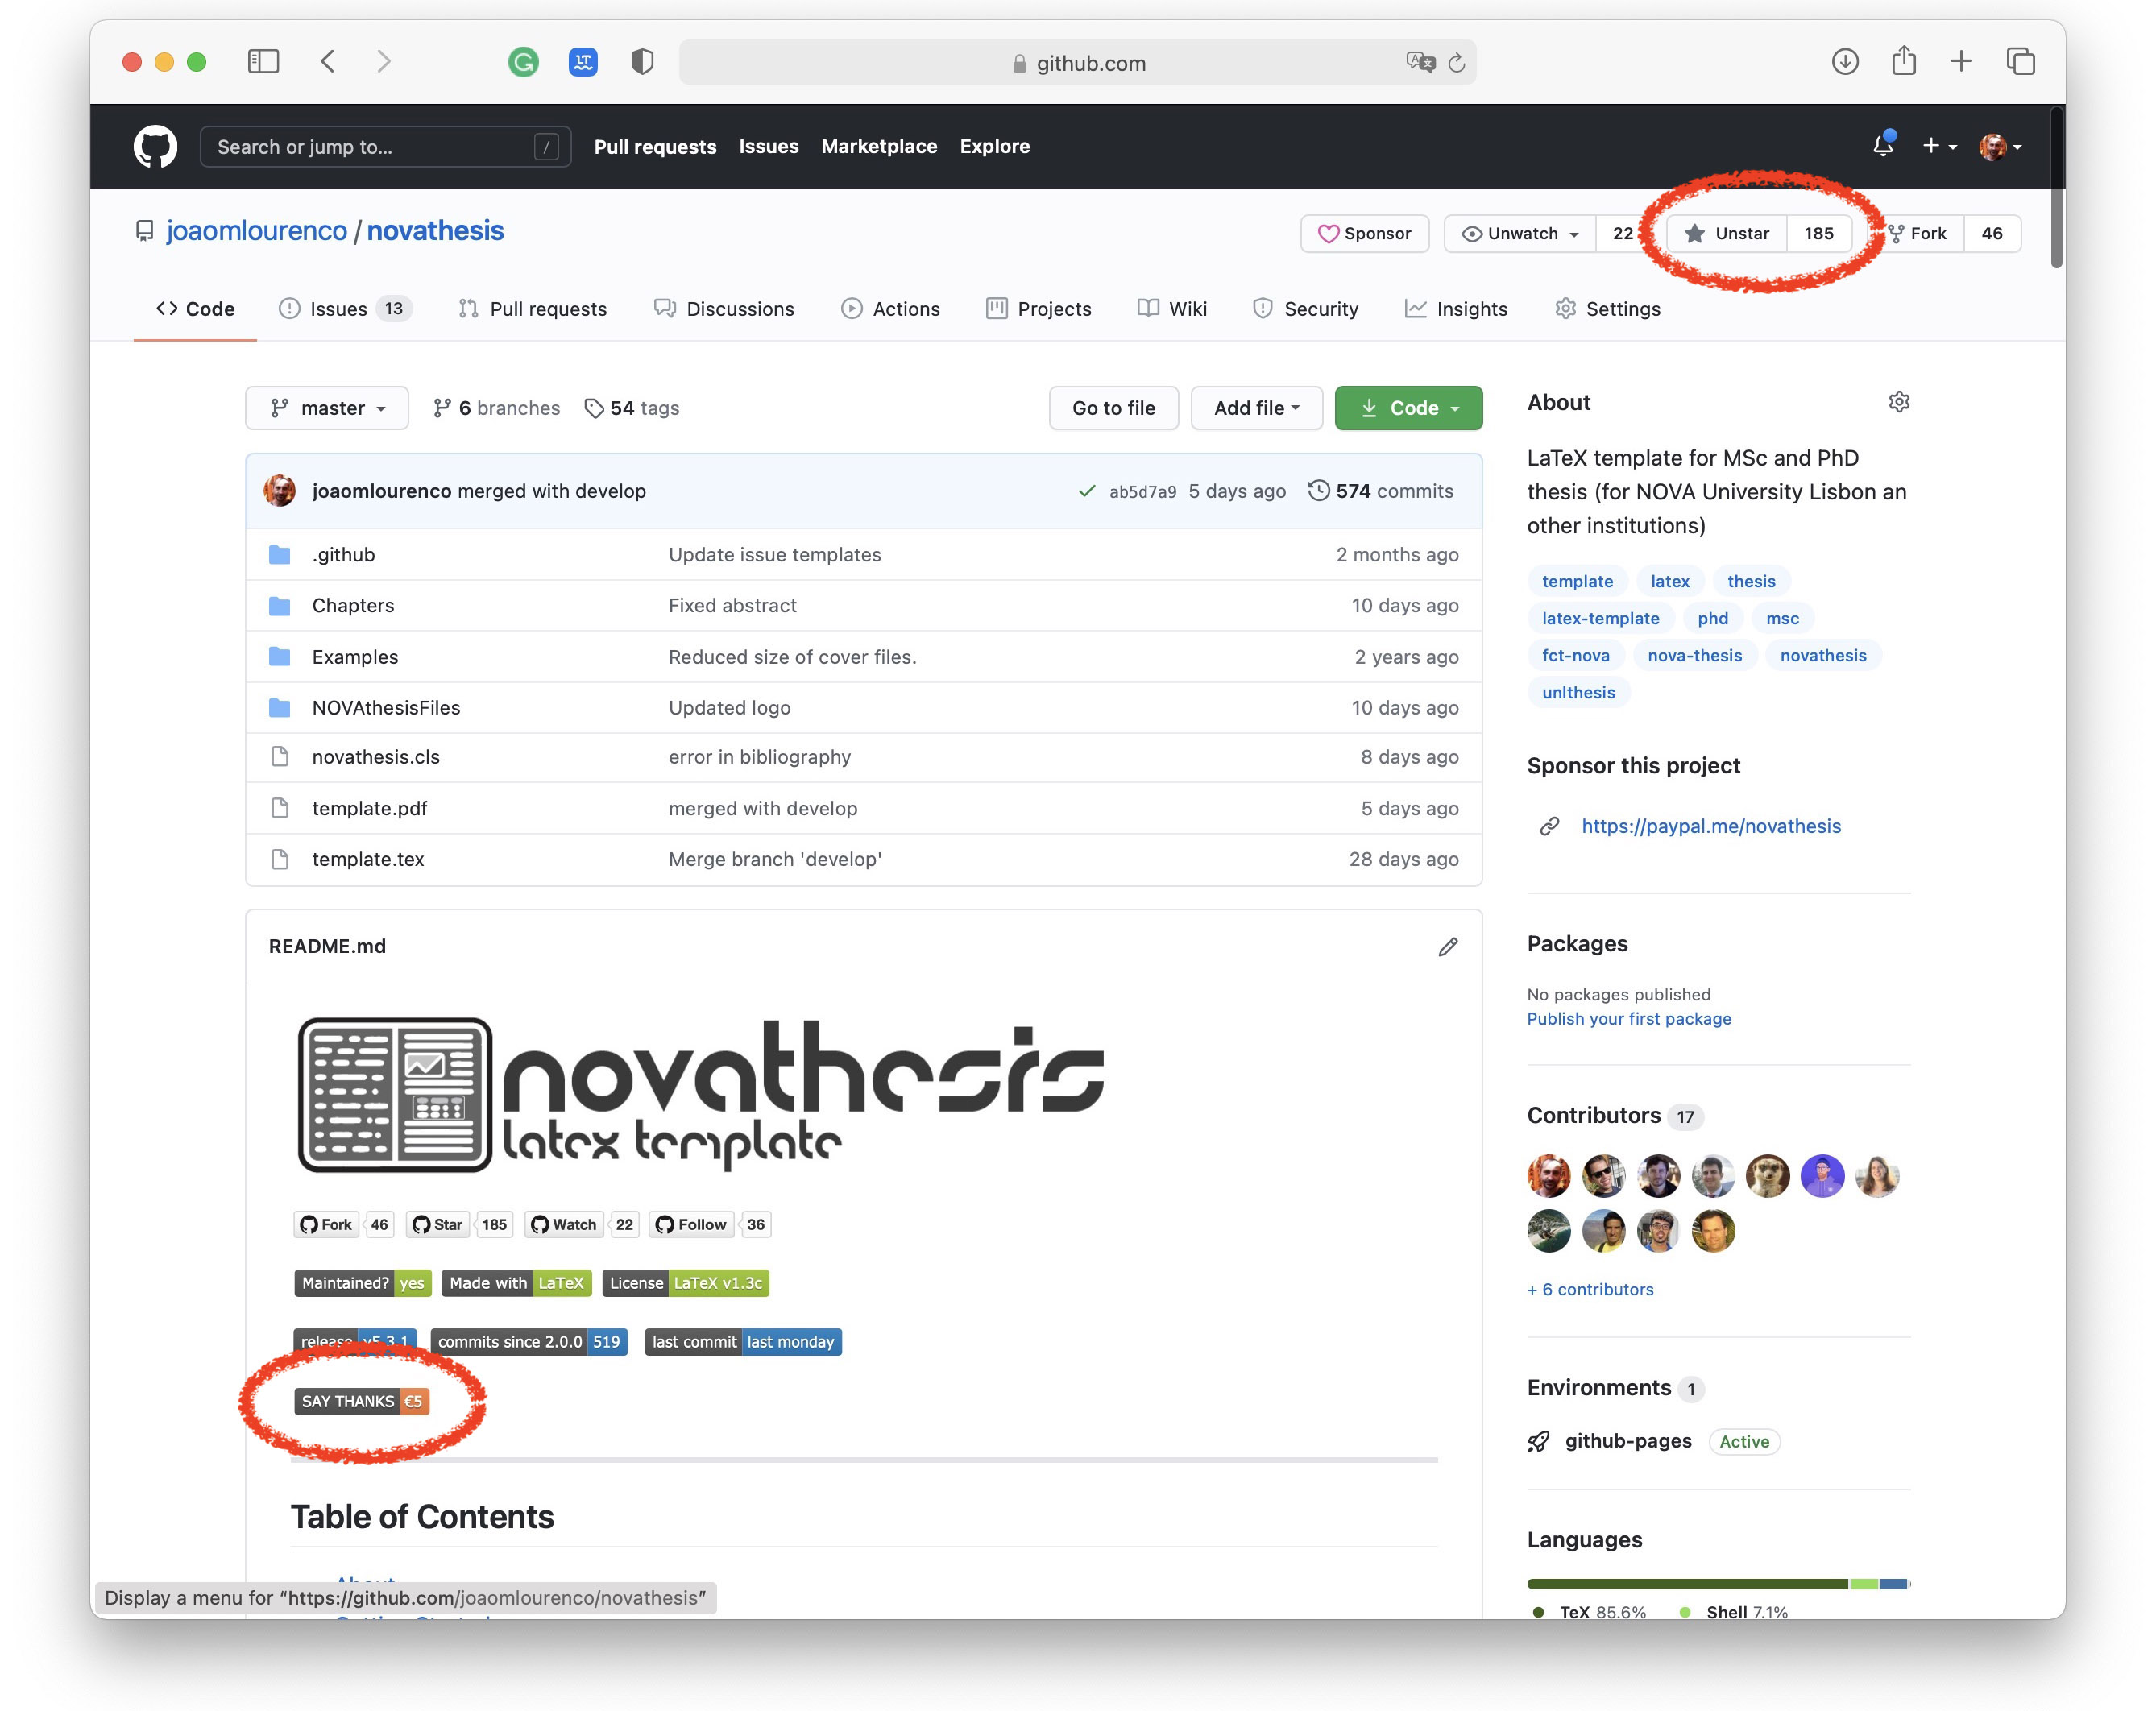
\includegraphics[width=\textwidth]{github1}
  \caption{The \novathesis{} project web page in GitHub.}
  \label{fig:github}
\end{figure}


\section{The \emph{NOVAthesis} template}
\label{sec:a_bit_of_history}

\newcommand{\mysmallcoversize}{0.09\linewidth}
\renewcommand{\theadfont}{\large\bfseries}
\definecolor{Schlgray}{gray}{0.95}  
\newtoggle{ntRow}

\newcommand{\ntSchool}[4]{%
    % #1 = cover image
    % #2 = School name
    % #3 = School acronym
    % #3 = School URL
    \iftoggle{ntRow}{\rowcolor{GhostWhite}\global\togglefalse{ntRow}}{\global\toggletrue{ntRow}}
    \setlength{\fboxsep}{0pt}%
    \makecell*[cc]{\fbox{\colorbox{White}{\includegraphics[width=\mysmallcoversize]{#1}}}}
    & #2 \href{#4}{(#3)}\\%
}

\newenvironment{ntUnivesity}[1]{
    \togglefalse{ntRow}
    \xltabular{\linewidth}{lX}%
    \toprule%
    \rowcolor{Gainsboro}%
    & \Gape[1.5ex]{\thead[l]{#1}}\\
    \midrule%
}{%
    \bottomrule
    \endxltabular%
}

The \gls{novathesis} was initially directed to the PhD and MSc students thesis at \gls{DI} of the \gls{FCT} of the \gls{NOVA}, Portugal, but currently it supports other Universities and Schools, namely:

\begin{ntUnivesity}{NOVA University Lisbon}
    \ntSchool{cover-nova-fct-phd}%
                  {NOVA School of Science and Technology}%
                  {FCT-NOVA}%
                  {https://www.fct.unl.pt}
    \ntSchool{cover-nova-fcsh-phd}%
                  {NOVA School of Social Sciences and Humanities}%
                  {FCSH-NOVA}%
                  {https://www.fcsh.unl.pt}
    \ntSchool{cover-nova-ims-phd}%
                  {NOVA Information Management School}%
                  {NOVA-IMS}%
                  {https://www.novaims.unl.pt}
    \ntSchool{cover-nova-ensp-phd}%
                  {National School of Public Heath}%
                  {ENSP-NOVA}%
                  {https://www.ensp.unl.pt}
\end{ntUnivesity}

\begin{ntUnivesity}{University of Lisbon}
    \ntSchool{cover-ul-ist-phd}%
                  {Instituto Superior Técnico}%
                  {IST-UL}%
                  {https://tecnico.ulisboa.pt}
    \ntSchool{cover-ul-fc-phd}%
                  {Faculdade de Ciências}%
                  {FCUL}%
                  {https://ciencias.ulisboa}
\end{ntUnivesity}

\begin{ntUnivesity}{University of Minho}
    \ntSchool{cover-uminho-ea-phd}%
                  {Escola de Arquitetura}%
                  {EA-UM}%
                  {https://www.arquitetura.uminho.pt}
    \ntSchool{cover-uminho-ec-phd}%
                  {Escola de Ciências}%
                  {EC-UM}%
                  {https://www.ecum.uminho.pt}
    \ntSchool{cover-uminho-ed-phd}%
                  {Escola de Direito}%
                  {ED-UM}%
                  {https://www.direito.uminho.pt}
    \ntSchool{cover-uminho-eeg-phd}%
                  {Escola de Economia e Gestão}%
                  {EEG-UM}%
                  {https://www.eeg.uminho.pt}
    \ntSchool{cover-uminho-ee-phd}%
                  {Escolha de Engenharia}%
                  {EE-UM}%
                  {https://www.eng.uminho.pt}
    \ntSchool{cover-uminho-em-phd}%
                  {Escola de Medicina}%
                  {EM-UM}%
                  {https://www.med.uminho.pt}
    \ntSchool{cover-uminho-ep-phd}%
                  {Escola de Psicologia}%
                  {EP-UM}%
                  {https://www.psi.uminho.pt}
    \ntSchool{cover-uminho-ese-phd}%
                  {Escola Superior de Enfermagem}%
                  {ESE-UM}%
                  {https://www.ese.uminho.pt}
    \ntSchool{cover-uminho-ics-phd}%
                  {Instituto de Ciências Sociais}%
                  {ICS-UM}%
                  {https://www.ilch.uminho.pt}
    \ntSchool{cover-uminho-ie-phd}%
                  {Instituto de Educação}%
                  {IE-UM}%
                  {https://www.ie.uminho.pt}
    \ntSchool{cover-uminho-ilch-phd}%
                  {Instituto de Letras e Ciências Humanas}%
                  {ILCH-UM}%
                  {https://www.ilch.uminho.pt}
    \ntSchool{cover-uminho-i3b-phd}%
                  {Instituto de Investigação em Biomateriais, Biodegradáveis e Biomiméticos}%
                  {I3B-UM}%
                  {https://i3bs.uminho.pt}
\end{ntUnivesity}

\begin{ntUnivesity}{ISCTE — Instituto Universitário de Lisboa}
    \ntSchool{cover-iscte-iul-eta-phd}%
             {Escola de Tecnologias e Arquitectura}%
             {ETA-ISCTE-IUL}%
             {https://ciencia.iscte-iul.pt/schools/escola-tecnologias-arquitectura}%
\end{ntUnivesity}

\begin{ntUnivesity}{Instituto Politécnico de Lisboa}
    \ntSchool{cover-ipl-isel-phd}%
             {Instituto Superior de Engenharia de Lisboa}%
             {ISEL-IPL}%
             {https://www.isel.pt}%
\end{ntUnivesity}

\begin{ntUnivesity}{Instituto Politécnico de Setúbal}
    \ntSchool{cover-ips-ests-phd}%
             {Escola Superior de Tecnologia de Setúbal}%
             {ISEL-IPL}%
             {https://www.estbarreiro.ips}%
\end{ntUnivesity}

\begin{ntUnivesity}{Other Universities/Schools/Degrees}
    \ntSchool{cover-other-esep-phd}%
             {Escola Superior de Enfermagem do Porto}%
             {ESEP}%
             {https://www.esenf.pt/pt}%
    \ntSchool{cover-other-gt-msc}%
             {Masters Program in Geospatial Technologies}%
             {GT}%
             {https://mastergeotech.info}%
\end{ntUnivesity}


\section{Getting Started}
\label{sec:getting_started}

The template provides an \emph{easy to use} setting for you to write your thesis/dissertation in \LaTeX:
\begin{itemize}
  \item  Select your school;
  \item Fill your thesis metadata (title, research field, etc) in the file “\texttt{template.tex}”;
  \item Create your thesis/dissertation contents using the files in folder “\texttt{Chapters}”; and
  \item Process using you favorite \LaTeX\ processor (pdf\LaTeX, \XeLaTeX\ or \LuaLaTeX).
\end{itemize}

\subsection{Using Overleaf}
\label{sub:using_overleaf}

\begin{wrapfigure}{r}{0.5\linewidth}
\vspace*{-15ex}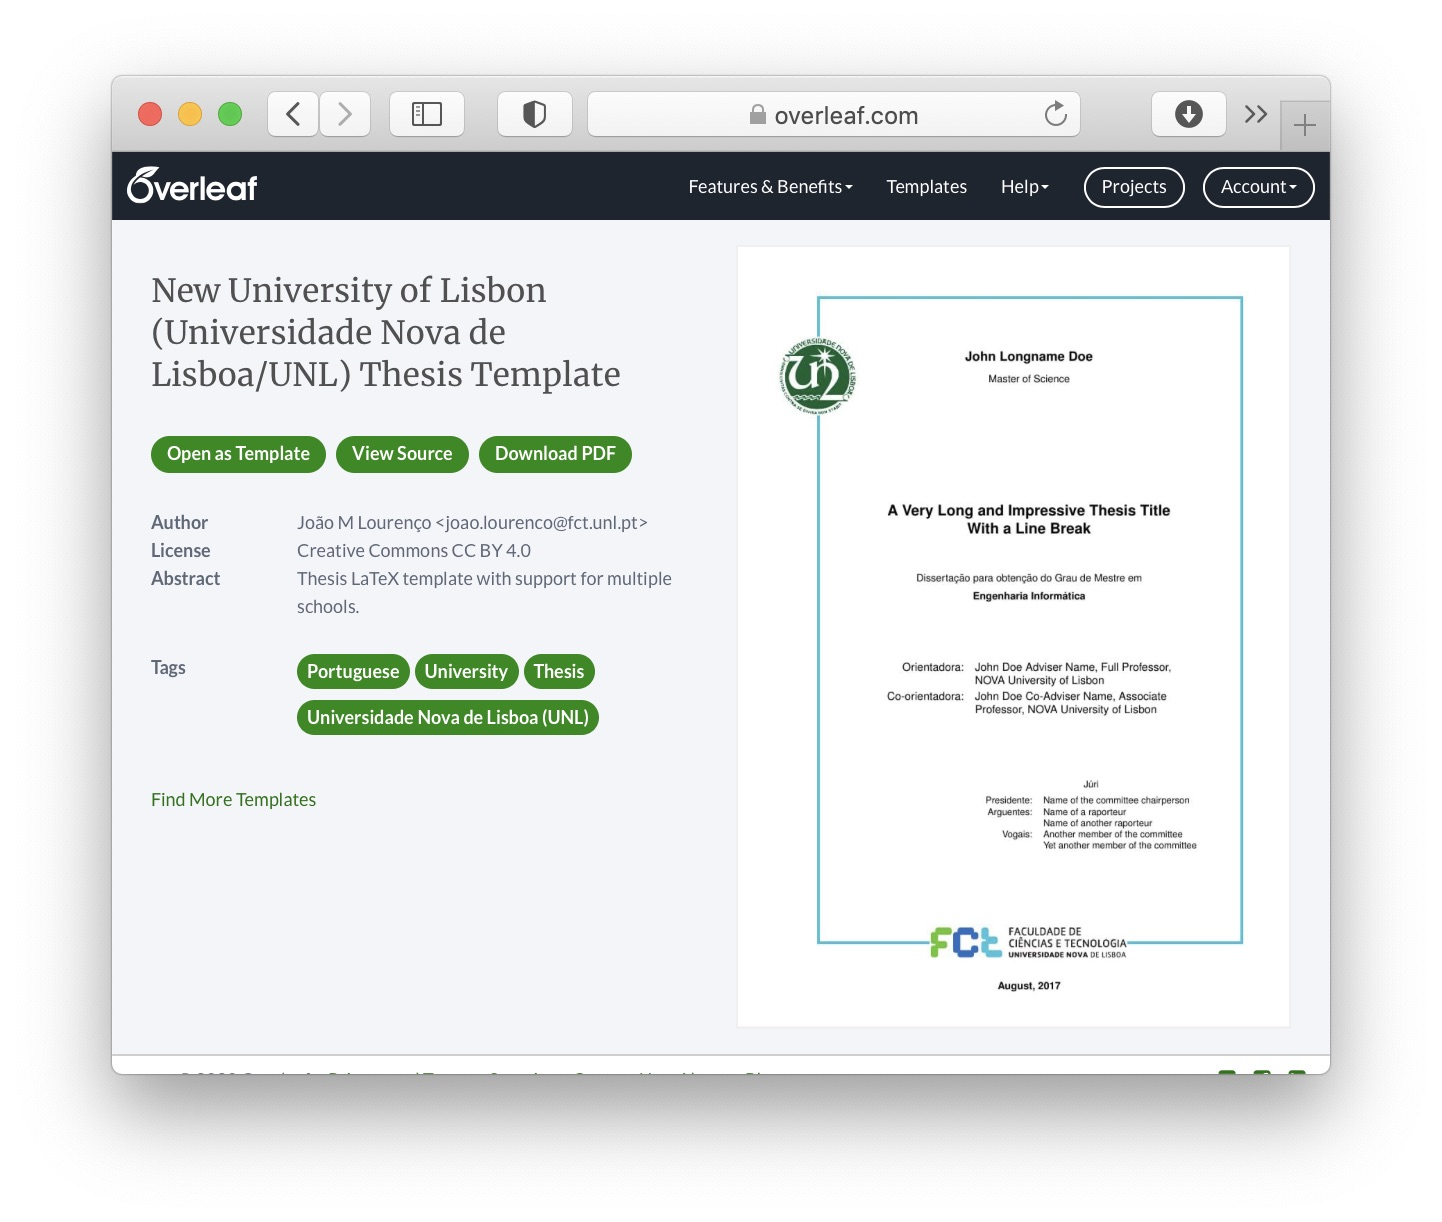
\includegraphics[width=\linewidth]{overleaf}%
\end{wrapfigure}

If you do not have an account in \href{https://www.overleaf.com?r=f5160636&rm=d&rs=b}{Overleaf}, you must \href{https://www.overleaf.com?r=f5160636&rm=d&rs=b}{create one first}.

Once you have an account, please access the \glsxtrlong{novathesis} in \href{https://www.overleaf.com/latex/templates/new-university-of-lisbon-universidade-nova-de-lisboa-slash-unl-thesis-template/fwbztcrptjmg}{Overleaf} and select the green button \emph{Open as Template}. 

\emph{Please note that the version currently available in Overleaf (v4.1.3) is outdated. A new version will be submitted to Overleaf soon.}  

\subsection{Using a Local \LaTeX\ Installation}
\label{sub:using_local_latex}

\begin{wrapfigure}{r}{0.5\linewidth}
\vspace*{-15ex}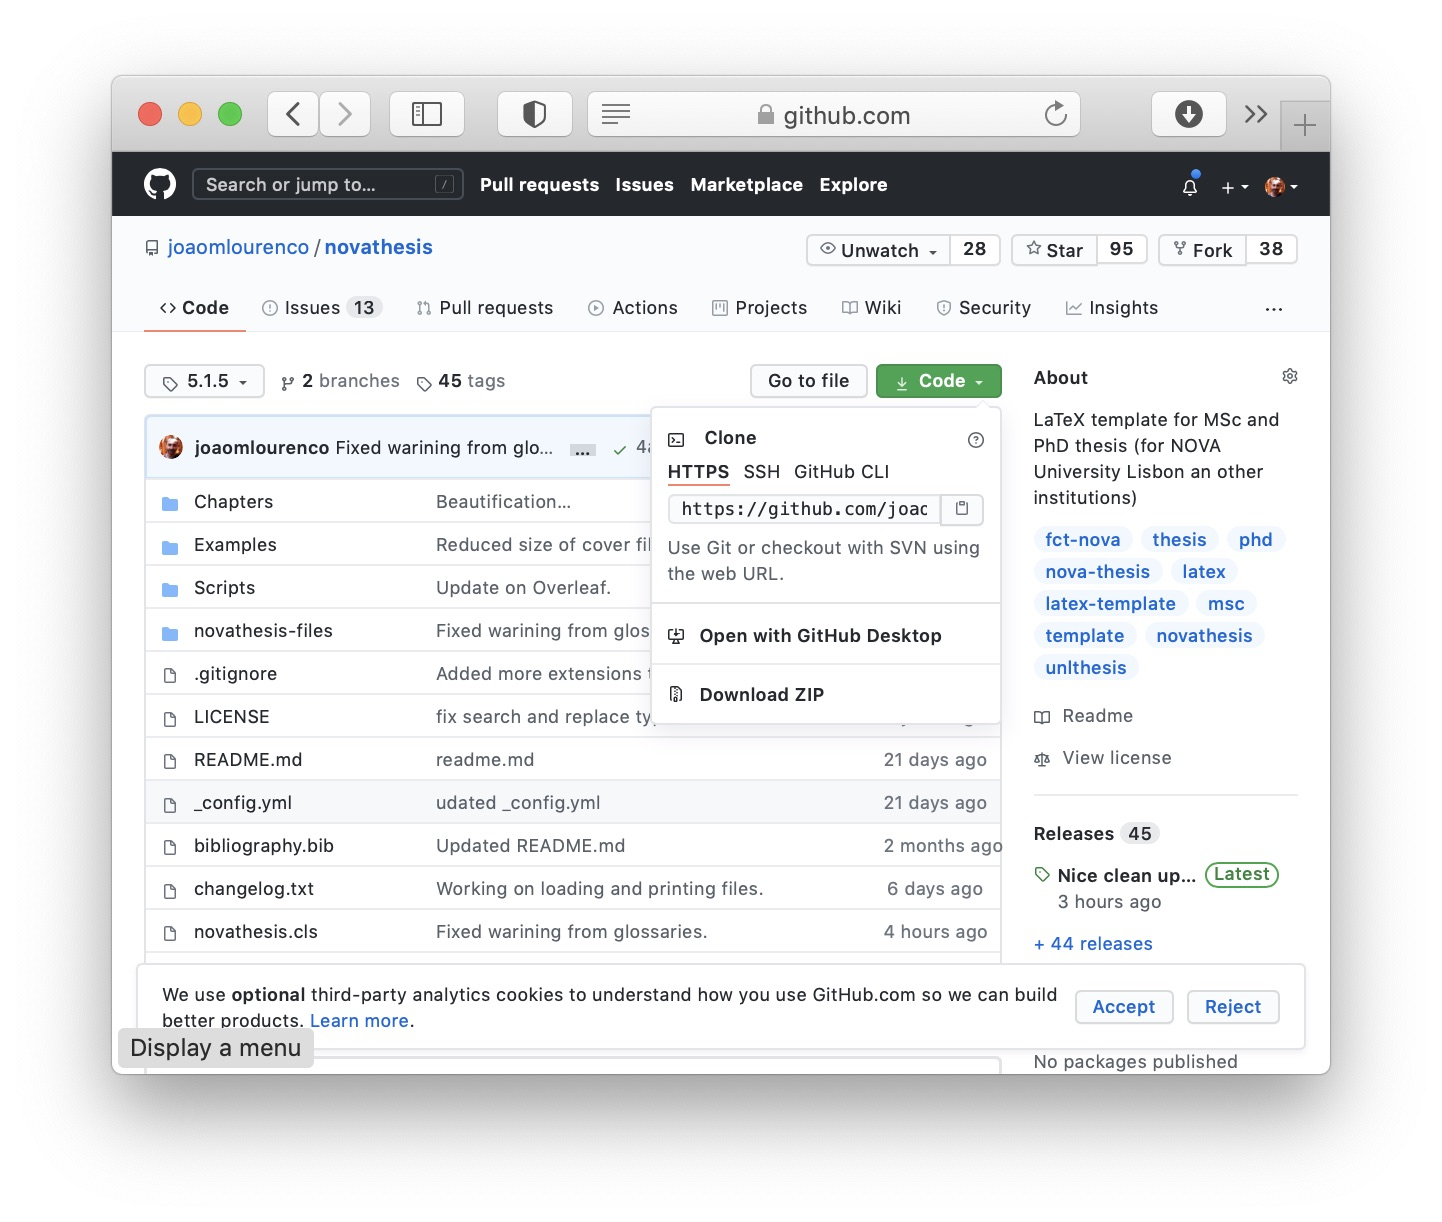
\includegraphics[width=\linewidth]{github}%
\end{wrapfigure}

Just access the \glsxtrlong{novathesis} in \href{https://github.com/joaomlourenco/novathesis}{GitHub}, select the green button \emph{Code} and then \emph{download} (or \emph{clone}) the template.  You will always get the latest version of the template (currently v5.1.8).


\section{Getting Help}
\label{sec:getting_help}

\begin{center}  
  \fbox{\textbf{Please do not send me emails!  I will not answer them!}}
\end{center}
 
\subsection{Google}
\label{sub:group_google}

Remember, when looking for hints or help, \emph{\href{google.com}{Google} is your best friend}!   And if you prefix your Google query with “\emph{LaTeX}”, your fist link will most probably direct you to \texttt{tex.stackexchange.com}.

\subsection{Group Support}
\label{sub:group_support}

To get directed help on the \glsxtrlong{novathesis} please join:
\begin{itemize}
  \item the \href{https://www.facebook.com/groups/novathesis}{NOVAtheis Facebook group}, or
  \item the \href{https://groups.google.com/forum/#!forum/novathesis}{NOVAthesis Google group}.
\end{itemize}

There were huge changes from version 4.x.y to version 5.a.b so, please, \textbf{always} state the version number you are using when asking for help.

\subsection{Reporting Problems}
\label{sub:reporting_problems}

If you just need some help, see above \Autoref{sub:group_google} and \Autoref{sub:group_support}.

If you believe \emph{you found a bug} or if \emph{you need some improvement} in the template, please \href{https://github.com/joaomlourenco/novathesis/issues}{fill an issue in github} at \url{https://github.com/joaomlourenco/novathesis/issues}.


\section{Donations}
\label{sec:donations}

This template is the result of hundreds (yes! \emph{may hundreds}!) of hours of work from the \href{https://docentes.fct.unl.pt/joao-lourenco}{main developer}.  If you think this template really made you life easier while writing your thesis, please consider \href{https://paypal.me/novathesis}{\textbf{making a donation}}. We will keep a list thanking to all the identified donors that identify themselves in the “\emph{Add special instructions to the seller}” box.

\subsubsection*{Donors 2020}
\label{ssub:donors_2020}

\begin{inparaitem}[]
  \item João Carvalho, 
  \item David Romão, 
  \item DisplayersereStream, and
  \item António Estêvão.  
\end{inparaitem}

\subsubsection*{Donors 2019}
\label{ssub:donors_2019}

\begin{inparaitem}[]
  \item Jorge Barreto and
  \item Raissa Almeida.  
\end{inparaitem}



\section{Disclaimer}
\label{sec:disclaimer}

Although this template is endorsed by the FCT-NOVA and even \href{https://www.fct.unl.pt/estudante/informacao-academica}{linked from its web site}, this is still not an official template.
%
This template exists to make your life easier and we do our best to make the \gls{novathesis} template compliant to the supported Schools' regulations, but in the end of the line you and only you are accountable for both the look and the contents of the document you submit as your thesis/dissertation.

% \printbibliography[heading=subbibliography, segment=\therefsegment, title={\bibname\ for chapter~\thechapter}]
